% =====================================================================
%  INFORME TÉCNICO — PROYECTO FINAL DE INTELIGENCIA ARTIFICIAL
%  Clasificación con MLP (datos tabulares) y CNN (imágenes)
%  Referencia principal: James et al. (2023) ISLP, Caps. 2, 4 y 10
%
%  COMPILACIÓN (ejecutar desde la carpeta latex/):
%    pdflatex main.tex && bibtex main && pdflatex main.tex && pdflatex main.tex
%
%  IMÁGENES REQUERIDAS en la misma carpeta:
%    loss_tabular.png   (curva de pérdida MLP)
%    loss_cnn.png       (curva de pérdida CNN)
%    conf_matrix.png    (matriz de confusión CNN)
% =====================================================================
\documentclass[12pt, a4paper]{article}

% ── Codificación y fuente ─────────────────────────────────────────────
\usepackage[utf8]{inputenc}
\usepackage[T1]{fontenc}
\usepackage{babel}

% ── Matemáticas ───────────────────────────────────────────────────────
\usepackage{amsmath}
\usepackage{amssymb}
\usepackage{bm}

% ── Figuras y tablas ──────────────────────────────────────────────────
\usepackage{graphicx}
\usepackage{booktabs}
\usepackage{float}
\usepackage{caption}
\usepackage{subcaption}
\usepackage{array}

% ── Diseño de página ──────────────────────────────────────────────────
\usepackage[left=2.5cm, right=2.5cm, top=3cm, bottom=3cm]{geometry}
\usepackage{setspace}
\usepackage{parskip}
\setlength{\parindent}{0pt}
\setlength{\parskip}{8pt}

% ── Color y código ────────────────────────────────────────────────────
\usepackage{xcolor}
\usepackage{listings}
\lstset{
  basicstyle=\ttfamily\small,
  backgroundcolor=\color{gray!10},
  frame=single, rulecolor=\color{gray!40},
  numbers=left, numberstyle=\tiny\color{gray},
  breaklines=true, language=Python,
  keywordstyle=\color{blue!80!black},
  commentstyle=\color{green!55!black},
  stringstyle=\color{orange!80!black}
}

% ── Encabezado y pie de página ────────────────────────────────────────
\usepackage{fancyhdr}
\pagestyle{fancy}
\fancyhf{}
\rhead{\small Proyecto Final --- Inteligencia Artificial}
\lhead{\small MLP y CNN con PyTorch \textbar\ ISLP 2023}
\cfoot{\small\thepage}
\renewcommand{\headrulewidth}{0.4pt}
\setlength{\headheight}{15pt}

% ── Hipervínculos ─────────────────────────────────────────────────────
\usepackage[colorlinks=true,
            linkcolor=blue!70!black,
            citecolor=blue!70!black,
            urlcolor=blue!80!black]{hyperref}

% ── Bibliografía ──────────────────────────────────────────────────────
\usepackage{natbib}
\bibliographystyle{plainnat}

% ── Macros matemáticas ────────────────────────────────────────────────
\newcommand{\X}{\mathbf{X}}
\newcommand{\W}{\mathbf{W}}
\newcommand{\bh}{\mathbf{h}}
\newcommand{\R}{\mathbb{R}}
\newcommand{\Loss}{\mathcal{L}}
\newcommand{\relu}{\text{ReLU}}
\DeclareMathOperator*{\argmin}{arg\,min}

% ── Metadatos PDF ────────────────────────────────────────────────────
\hypersetup{
  pdftitle={Informe Técnico: Clasificación con MLP y CNN},
  pdfauthor={Cristian Bravo},
  pdfsubject={Proyecto Final de Inteligencia Artificial},
  pdfkeywords={MLP, CNN, PyTorch, ISLP, Clasificacion}
}

% =====================================================================
\begin{document}

% ── Portada ──────────────────────────────────────────────────────────
\begin{titlepage}
  \centering
  \vspace*{1.2cm}

  {\large \textbf{Universidad Nacional de Colombia}}\\[0.3cm]
  {\normalsize Facultad de Ingeniería y Adminitración}\\[0.2cm]
  {\normalsize Inteligencia Artificial para la Agroindustria}\\[2.2cm]

  \rule{\linewidth}{1pt}\\[0.5cm]
  {\LARGE \textbf{Clasificación con Redes Neuronales Profundas}}\\[0.4cm]
  {\Large Componente Tabular (MLP) y Componente de Imágenes (CNN)}\\[0.4cm]
  {\normalsize Basado en \textit{An Introduction to Statistical Learning
    with Applications in Python} \citep{islp2023}}\\[0.4cm]
  \rule{\linewidth}{1pt}\\[2.0cm]

  \begin{minipage}{0.48\textwidth}
    \centering
    \textbf{Estudiante de Ingeniría Agronómica}\\[0.2cm]
    Cristian Andres Bravo Narvaez\\[0.1cm]
    {\small \texttt{cbravon@unal.edu.co}}
  \end{minipage}
  \hfill
  \begin{minipage}{0.48\textwidth}
    \centering
    \textbf{Docente}\\[0.2cm]
    John Jairo Leal Gomez\\[0.1cm]
    {\small Facultad de Ingeniería y Administración}
  \end{minipage}

  \vfill
  {\normalsize \today}
\end{titlepage}

% ── Resumen ──────────────────────────────────────────────────────────
\begin{abstract}
\noindent
Este informe describe la implementación y evaluación de dos
arquitecturas de redes neuronales profundas para problemas de
clasificación supervisada: un Perceptrón Multicapa (MLP) aplicado al
conjunto de datos tabulares \texttt{phpnThNfi.arff} (4\,839
instancias, 2 clases), y una Red Neuronal Convolucional (CNN) aplicada
al dataset \texttt{potato\_subset} (456 imágenes RGB, 3 clases de
enfermedades en papa). Ambos modelos fueron implementados en Python
con PyTorch, siguiendo los principios metodológicos del libro
\textit{An Introduction to Statistical Learning with Applications in
Python} \citep{islp2023}. El MLP alcanzó una \textit{accuracy} del
\textbf{98.86\%} y la CNN del \textbf{94.57\%}. Se analizan las
decisiones de diseño de la arquitectura, el preprocesamiento de datos,
las estrategias de regularización y las métricas de evaluación,
conectando cada decisión con los temas estudiados en el curso.
\end{abstract}

\newpage
\tableofcontents
\newpage

% =====================================================================
\section{Introducción}
\label{sec:intro}
% =====================================================================

El presente proyecto final integra los conceptos teóricos y prácticos
estudiados a lo largo del curso de Inteligencia Artificial, cubriendo
desde los fundamentos del aprendizaje estadístico supervisado hasta la
implementación de redes neuronales profundas. El trabajo se organiza
en dos componentes complementarios:

\textbf{Componente Tabular.} Se trabaja con el archivo
\texttt{phpnThNfi.arff}, un conjunto de datos en formato ARFF
(\textit{Attribute-Relation File Format}) compuesto por 4\,839
registros con cinco variables numéricas de entrada ($V_1, \ldots, V_5$)
y una variable objetivo binaria (\texttt{Class} $\in \{1, 2\}$). La
distribución de clases es marcadamente desbalanceada: 94.6\% clase~1
(916 instancias en test) frente al 5.4\% clase~2 (52 instancias en
test). La tarea consiste en desarrollar un modelo de clasificación
empleando una Red Neuronal Multicapa (MLP).

\textbf{Componente de Imágenes.} Se emplea el dataset
\texttt{potato\_subset}, que contiene 456 imágenes RGB de hojas de
papa clasificadas en tres categorías: \textit{Early Blight} (tizón
temprano), \textit{Late Blight} (tizón tardío) y \textit{Healthy}
(saludable). El subconjunto proviene de un conjunto más grande de
imágenes de enfermedades foliares. La tarea es desarrollar un modelo
de clasificación mediante una Red Neuronal Convolucional (CNN).

Ambos modelos fueron implementados en Python con PyTorch, entregados
en GitHub y documentados en este informe compilado en \LaTeX, tal como
se indicó en los requerimientos del proyecto:
comprensión del problema, explicación matemática del método,
explicación conceptual del funcionamiento, ejemplo de apoyo,
implementación con PyTorch y evaluación de resultados.

% =====================================================================
\section{Temas Estudiados: Marco Teórico}
\label{sec:teoria}
% =====================================================================

\subsection{Capítulo 2 -- Aprendizaje Estadístico}
\label{subsec:cap2}

\subsubsection{¿Qué es el aprendizaje estadístico?}

El aprendizaje estadístico es un conjunto de enfoques para estimar
$f$ (modelo predictivo), que engloba el aprendizaje automático
supervisado \citep[Cap.~2]{islp2023}. La motivación fundamental
proviene de la relación entre variables predictoras y una respuesta.
Por ejemplo, la asociación entre publicidad (TV, radio, periódico)
y ventas en 200 mercados:

\begin{equation}
  Y = f(\X) + \varepsilon,
  \qquad \X = (X_1, X_2, \ldots, X_p),
  \label{eq:modelo_estadistico}
\end{equation}

donde $f$ es la función desconocida a estimar, $\varepsilon$ es el
error aleatorio con $\bar{\varepsilon} \approx 0$, e $Y$ es la
respuesta. El aprendizaje estadístico proporciona el conjunto de
enfoques para estimar $f$ (modelo predictivo), siendo el ML supervisado
el más relevante para este proyecto.

\textbf{Aprendizaje supervisado.} Para cada observación de las
mediciones predictoras $X_i$, $i = 1, \ldots, n$, existe una medición
de respuesta asociada $Y_i$. El modelo relaciona la respuesta con los
predictores con el objetivo de predecir la respuesta para futuras
observaciones. Los métodos clásicos incluyen Regresión Lineal y
Regresión Logística, así como enfoques modernos como GAM (Modelos
Aditivos Generalizados), Boosting y SVM (Máquinas de Vectores de
Soporte).

\subsubsection{¿Por qué estimar \texorpdfstring{$f$}{f}?}

Existen dos razones principales para estimar $f$:
predicción e inferencia \citep[Sec.~2.1]{islp2023}.

\textbf{Predicción.} Cuando el conjunto de entrada $X$ produce una
salida $Y$ que no se obtiene con facilidad, se estima $\hat{f}$ tal
que:
\begin{equation}
  \hat{Y} = \hat{f}(\X).
  \label{eq:prediccion}
\end{equation}
La precisión de $\hat{Y}$ como predicción de $Y$ depende del
\textit{error reducible} (que podemos minimizar mediante mejores
técnicas de aprendizaje) y del \textit{error irreducible} (inherente
al problema: $Y = f(\X) + \varepsilon$). Por tanto:
\begin{equation}
  E(Y - \hat{Y})^2 = \underbrace{[f(\X) - \hat{f}(\X)]^2}_{\text{Error reducible}}
  + \underbrace{\mathrm{Var}(\varepsilon)}_{\text{Error irreducible}}.
  \label{eq:error_descomp}
\end{equation}

\textbf{Inferencia.} La necesidad de conocer la relación entre $Y$ y
$X_1, X_2, \ldots, X_p$, estimando $f$ no para predicciones sino para
entender: ¿qué predictores están asociados a la respuesta?, ¿cuál
es la relación entre la respuesta y cada predictor?, ¿puede modelarse
la relación entre $Y$ y $X$ mediante una ecuación lineal?

\subsubsection{¿Cómo estimamos \texorpdfstring{$f$}{f}?}

Se asume que hemos observado un conjunto de $n$ puntos de datos
distintos (datos de entrenamiento), que usamos para entrenar o enseñar
a nuestro método a estimar $f$ \citep[Sec.~2.1.3]{islp2023}.

\textbf{Métodos paramétricos.} Enfoque basado en dos pasos:
\begin{enumerate}
  \item Se hace una suposición sobre la forma funcional de $f$.
    Por ejemplo, una suposición muy simple es que $f$ es lineal en $X$:
    \begin{equation}
      f(X) = \beta_0 + \beta_1 X_1 + \beta_2 X_2 + \cdots + \beta_p X_p.
    \end{equation}
    En lugar de estimar una función arbitraria de $p$ dimensiones,
    solo necesitamos estimar los $p+1$ coeficientes.
  \item Después de seleccionar un modelo, necesitamos ajustar o
    entrenar el modelo. En el caso del modelo lineal, el enfoque más
    común se denomina mínimos cuadrados ordinarios.
\end{enumerate}

El modelo paramétrico puede no coincidir con la verdadera forma
desconocida de $f$. Los modelos flexibles requieren más parámetros
y pueden conducir a sobreajuste (\textit{overfitting}).

\textbf{Métodos no paramétricos.} No hacen suposiciones explícitas
sobre la forma funcional de $f$; buscan una estimación de $f$ lo más
cerca posible a los datos sin irregularidades. Requieren un número
grande de observaciones. Por ejemplo, \textit{thin-plate spline}
produce una estimación lo más cerca posible a los datos observados,
sujeta a un ajuste suave.

\subsubsection{Compromiso Sesgo-Varianza}

El error de predicción esperado puede descomponerse en tres
componentes fundamentales \citep[Sec.~2.2]{islp2023}:
\begin{equation}
  \mathbb{E}\bigl[(Y - \hat{f}(\X))^2\bigr] =
  \underbrace{\bigl[\mathrm{Sesgo}(\hat{f}(\X))\bigr]^2}_{\text{Sesgo}^2}
  + \underbrace{\mathrm{Var}\bigl(\hat{f}(\X)\bigr)}_{\text{Varianza}}
  + \underbrace{\mathrm{Var}(\varepsilon)}_{\text{Error irreducible}}.
  \label{eq:bias_variance}
\end{equation}

La forma en U observada en el MSE de prueba resulta de estas dos
propiedades en competencia. Los métodos más flexibles reducen el
error de entrenamiento pero pueden aumentar el error de prueba
(\textit{curva en V}). Este es el \textbf{criterio de flexibilidad}
clave en la selección de modelos.

El MSE se calcula usando los datos de entrenamiento con los que se
ajustó el modelo (MSE de entrenamiento). Sin embargo, nos interesa
realmente cuán bien funciona el método sobre datos de entrenamiento
--precisión de predicciones con datos de prueba:
$\mathrm{Ave}(y_0 - \hat{f}(x_0))^2$, donde $(x_0, y_0)$ es una
observación de prueba no utilizada en el experimento.

Cuando un método tiene bajo MSE de entrenamiento pero alto MSE de
prueba, se dice que está \textbf{sobreajustado} a los datos.
La solución es la \textbf{Validación Cruzada}.

% =====================================================================
\subsection{Capítulo 4 -- Clasificación}
\label{subsec:cap4}

\subsubsection{Regresión Logística}

La regresión logística modela la probabilidad de que $Y$ pertenezca
a una categoría particular. Para el conjunto de datos Default, la
respuesta cae en una de dos categorías: Sí o No
\citep[Cap.~4]{islp2023}.

Si la probabilidad de incumplimiento dado el saldo puede escribirse
como $\Pr(\textit{default} = \textit{Sí} \mid \textit{balance})$, se
abrevia como $p(\textit{balance}) = 0 \leq x \leq 1$. Si
$p(\textit{balance}) \geq 0.5$, se predice \textit{default} = Sí.

\subsubsection{Modelo Logístico}

Modelar $p(X) = \Pr(Y = 1 \mid X)$ usando la función logística:
\begin{equation}
  p(X) = \frac{e^{\beta_0 + \beta_1 X}}{1 + e^{\beta_0 + \beta_1 X}},
  \label{eq:logistica}
\end{equation}
lo que garantiza que las probabilidades estén siempre en $[0,1]$.
Reorganizando la ecuación~\eqref{eq:logistica}:
\begin{equation}
  \log\!\left(\frac{p(X)}{1-p(X)}\right) = \beta_0 + \beta_1 X.
  \label{eq:logodds}
\end{equation}
El término de la izquierda se llama \textit{log-odds} o
\textit{logit}. Los coeficientes se estiman por
máxima verosimilitud (\textit{maximum likelihood}).

\subsubsection{Función de Pérdida: Entropía Cruzada}

Para clasificación multiclase, la función de pérdida estándar es la
\textit{entropía cruzada} (\textit{cross-entropy loss})
\citep[Cap.~4]{islp2023}:
\begin{equation}
  \Loss(\theta) = -\frac{1}{n} \sum_{i=1}^{n} \sum_{k=1}^{K}
  y_{ik} \log\bigl(\hat{p}_{ik}\bigr),
  \label{eq:cross_entropy}
\end{equation}
donde $y_{ik} \in \{0,1\}$ es la codificación \textit{one-hot} de la
clase verdadera, y $\hat{p}_{ik}$ es la probabilidad predicha para la
clase $k$ en la observación $i$. Las probabilidades se obtienen
mediante la función \textit{Softmax}:
\begin{equation}
  \hat{p}_{ik} = \frac{\exp(z_{ik})}{\displaystyle\sum_{j=1}^{K} \exp(z_{ij})},
  \label{eq:softmax}
\end{equation}

\subsubsection{Regresión Logística Multinomial}

Para $K > 2$ clases, la codificación Softmax trata las $K$ clases de
forma simétrica, asumiendo $K = 1, \ldots, K$
\citep[Sec.~4.3]{islp2023}:
\begin{equation}
  \Pr(Y = k \mid X = x) =
  \frac{e^{\beta_{k0} + \beta_{k1}x_1 + \cdots + \beta_{kp}x_p}}
       {\displaystyle\sum_{\ell=1}^{K}
        e^{\beta_{\ell 0} + \beta_{\ell 1}x_1 + \cdots + \beta_{\ell p}x_p}}.
  \label{eq:softmax_multinomial}
\end{equation}

La log-odds relativa a la clase base $K'$ es:
\begin{equation}
  \log\!\left(\frac{\Pr(Y=k \mid X=x)}{\Pr(Y=K' \mid X=x)}\right) =
  (\beta_{k0} - \beta_{K'0}) + (\beta_{k1} - \beta_{K'1})x_1
  + \cdots + (\beta_{kp} - \beta_{K'p})x_p.
\end{equation}

En PyTorch, \texttt{nn.CrossEntropyLoss} integra \textit{log-softmax}
internamente por estabilidad numérica, por lo que la capa de salida
emite únicamente logits crudos.

\subsubsection{Métricas de Evaluación}

Para evaluar clasificadores, especialmente con clases desbalanceadas,
\citet[Cap.~4]{islp2023} recomiendan reportar:
\begin{itemize}
  \item \textbf{Accuracy}: de los totales, cuántos datos acertó.
  \item \textbf{Precision}: qué tan seguido ocurre el acierto positivo.
  \item \textbf{Recall}: de los casos reales, cuántos detectó.
  \item \textbf{F1-Score}: media armónica de Precisión y Recall.
\end{itemize}

% =====================================================================
\subsection{Capítulo 8 -- Árboles y Métodos de Conjunto}
\label{subsec:cap8}

\subsubsection{Árboles de Decisión -- Predicción por Estratificación}

La predicción mediante estratificación del espacio de características
consiste en dividir el espacio de predictores en un conjunto de valores
posibles en regiones. Para la observación en la región $R_j$, se hace
la misma predicción: la media de los valores de respuesta de las
observaciones de entrenamiento en $R_j$.

Los predictores producen rectángulos de alta dimensión por simplicidad
e interpretabilidad. Se encuentran los rectángulos $R_1, \ldots, R_J$
que minimizan la Suma de Residuos al Cuadrado (RSS):
\begin{equation}
  \sum_{j=1}^{J} \sum_{i \in R_j} (y_i - \hat{y}_{R_j})^2.
\end{equation}

Se adopta la \textbf{División Binaria Recursiva}: de arriba a abajo,
comienza en la cima y va dividiendo sucesivamente, seleccionando el
predictor $X_j$ y punto de corte $s$ tal que divida el espacio en las
regiones $\{X \mid X_j < s\}$ y $\{X \mid X_j \geq s\}$.

\subsubsection{Random Forest y Bosques Aleatorios}

Los árboles ensacados aleatorios superan el problema de correlación
entre árboles obligando a cada división a considerar solo un
subconjunto de los predictores $m$. Por tanto, en promedio,
$(p-m)/p$ no considera al predictor más fuerte, dando oportunidad
a otros predictores, decorrelacionando los árboles y produciendo
un promedio menos variable.

La diferencia entre árboles aleatorios y ensacados es la elección
del tamaño del subconjunto de predictores $m$. Si se construye un
bosque aleatorio usando $m = p$, esto equivale al ensacado. En los
datos Heart con $m = \sqrt{p}$, los bosques aleatorios conducen a
una reducción tanto en el error de prueba como en el error OOB
respecto al ensacado.

Random Forest es especialmente útil con conjuntos de datos
biológicos de alta dimensionalidad (por ejemplo, 4\,718 genes en
muestras de tejido de 349 pacientes con 15 tipos distintos de cáncer).

% =====================================================================
\subsection{Capítulo 10 -- Aprendizaje Profundo}
\label{subsec:cap10}

\subsubsection{Red Neuronal Multicapa (MLP)}

Un MLP de $L$ capas ocultas transforma la entrada mediante la
recurrencia \citep[Cap.~10]{islp2023}:
\begin{align}
  \bh^{(0)} &= \X, \nonumber \\
  \bh^{(\ell)} &= \sigma\!\left(\W^{(\ell)}\,\bh^{(\ell-1)}
    + \mathbf{b}^{(\ell)}\right),
    \quad \ell = 1,\ldots,L,
  \label{eq:mlp_forward} \\
  \hat{\mathbf{z}} &= \W^{(L+1)}\,\bh^{(L)}
    + \mathbf{b}^{(L+1)}. \nonumber
\end{align}

donde $g(z)$ es una función de activación no lineal, y $A_K$ es una
transformación diferente $h_K(X)$.

\textbf{Función de activación sigmoide:}
\begin{equation}
  g(z) = \frac{e^z}{1 + e^z} = \frac{1}{1 + e^{-z}}.
  \label{eq:sigmoide}
\end{equation}

\textbf{Función ReLU} (preferida en redes modernas):
\begin{equation}
  \relu(z) = g(z) = (z)_+ =
  \begin{cases} z & \text{si } z \geq 0, \\ 0 & \text{si } z < 0. \end{cases}
  \label{eq:relu}
\end{equation}

\citet[Cap.~10]{islp2023} destacan que ReLU es más conveniente y que
la no linealidad en la función de activación $g(z)$ es esencial:
sin ella, el modelo $f(X)$ se reduciría a un modelo lineal en
$X_1, \ldots, X_p$. La no linealidad permite capturar no linealidades
complejas y efectos de interacción.

\textbf{Arquitectura MNISTModel (referencia del libro):}
\begin{itemize}
  \item Capa 1: Aplanar (784 entradas) $\to$ Lineal$(784 \to 256)$
    $\to$ ReLU $\to$ Dropout$(40\%)$.
  \item Capa 2: Lineal$(256 \to 128)$ $\to$ ReLU $\to$ Dropout$(30\%)$.
  \item Salida: Lineal$(128 \to 10)$.
\end{itemize}
Modelo con 253\,146 parámetros, entrenado 30 épocas con entropía
cruzada en 256 observaciones -- 168 pasos por gradiente.

\subsubsection{Regularización por Dropout}

Para controlar el sobreajuste, se aplica \textit{Dropout Learning}
\citep[Sec.~10.7.3]{islp2023}: durante el entrenamiento, cada neurona
se desactiva aleatoriamente con probabilidad $p_d$:
\begin{equation}
  \tilde{h}^{(\ell)}_j =
  \frac{m_j^{(\ell)}}{1 - p_d}\cdot h^{(\ell)}_j,
  \quad m_j^{(\ell)} \sim \text{Bernoulli}(1 - p_d).
  \label{eq:dropout}
\end{equation}
Las redes neuronales son sensibles a la escala de las entradas
(Ridge y Lasso también son afectadas). Las entradas con valores de
escala de grises de 8 bits entre 0--255 se reescalan al intervalo
unitario $[0,1]$ mediante \texttt{ToTensor()}.

\subsubsection{Red Neuronal Convolucional (CNN)}

Las CNN explotan la estructura local de los datos en cuadrícula
mediante operaciones de convolución. Las capas de convolución usan
filtros: plantillas que determinan si una característica local
particular está presente en una imagen.

Se basan en una operación muy simple llamada convolución (multiplicar
elementos de matrices repetidamente y luego sumar resultados):

\begin{equation}
  (I * K)_{ij} = \sum_{m} \sum_{n}\, I_{(i+m)(j+n)} \cdot K_{mn}.
  \label{eq:convolucion}
\end{equation}

En una capa de convolución, se usa un banco completo de filtros para
detectar bordes y formas orientadas. En las CNN, los filtros se
aprenden para la tarea de clasificación específica.

\citet[Sec.~10.3.2]{islp2023} describen el \textit{MaxPooling} como
la operación que reduce la resolución espacial:
\begin{equation}
  \text{MaxPool}(I)_{ij} = \max_{(m,n)\in\mathcal{R}_{ij}} I_{mn}.
  \label{eq:maxpool}
\end{equation}

\textbf{Arquitectura CNN del proyecto (documentada en los apuntes):}
\begin{table}[H]
  \centering
  \small
  \setlength{\tabcolsep}{5pt}
  \renewcommand{\arraystretch}{1.2}
  \begin{tabular}{p{1.8cm} p{2.4cm} p{7.5cm} p{2.4cm}}
    \toprule
    \textbf{Bloque} & \textbf{Capa} & \textbf{Operación} & \textbf{Salida} \\
    \midrule
    Entrada      & --               & Imagen RGB $128\times128$
                   & $3\times128\times128$ \\
    Conv 1       & Bordes, Texturas & Conv(32) + BN + ReLU + MaxPool
                   & $32\times64\times64$ \\
    Conv 2       & Texturas, Formas & Conv(64) + BN + ReLU + MaxPool
                   & $64\times32\times32$ \\
    Conv 3       & Patrones         & Conv(128) + BN + ReLU + MaxPool
                   & $128\times16\times16$ \\
    Clasificador & FC               & Flatten(32768) + Linear(512) +
                   Dropout(0.5) + Linear(3) & 3 logits \\
    \bottomrule
  \end{tabular}
\end{table}

\textbf{Métricas de evaluación de la CNN:}
\begin{itemize}
  \item \textbf{Macro avg}: $\frac{\sum F_1}{3}$ -- cada clase es igual.
  \item \textbf{Weighted avg}: pondera $F_1$ por cuántas fotos tiene
    cada clase del total. Las clases con más fotos valen más.
\end{itemize}

% =====================================================================
\section{Metodología: Componente Tabular (MLP)}
\label{sec:metodo_tabular}
% =====================================================================

\subsection{Carga y exploración de datos}

El archivo \texttt{phpnThNfi.arff} fue cargado con
\texttt{scipy.io.arff.loadarff()}, función que preserva el tipo de
cada atributo definido en la cabecera ARFF. Las cadenas de bytes
resultantes fueron decodificadas a \texttt{str}. El conjunto final
contiene 4\,839 instancias, 5 variables numéricas de entrada y una
variable objetivo binaria (\texttt{Class} $\in \{1, 2\}$). La
variable objetivo fue codificada con \texttt{LabelEncoder} a enteros
$\{0, 1\}$, requeridos por la función de pérdida
\texttt{nn.\allowbreak CrossEntropyLoss}.

\subsection{Preprocesamiento}

El preprocesamiento siguió dos pasos:

\textbf{Partición 80/20.} Los datos fueron divididos con
\texttt{train\_test\_split} de \texttt{scikit-learn} usando muestreo
estratificado (\texttt{stratify=y}), garantizando que la proporción de
clases se preserve en ambas particiones. Se obtuvo un conjunto de
entrenamiento con 3\,871 instancias y uno de prueba con 968.

\textbf{Normalización (StandardScaler).} Las variables de entrada
fueron estandarizadas a media cero y desviación estándar unitaria:
\begin{equation}
  \tilde{x}_{ij} = \frac{x_{ij} - \bar{x}_j}{\hat{\sigma}_j},
  \label{eq:standardscaler}
\end{equation}
donde $\bar{x}_j$ y $\hat{\sigma}_j$ son la media y la desviación
estándar de la $j$-ésima variable, calculadas \emph{exclusivamente}
sobre el conjunto de entrenamiento. Aplicar la transformación sobre el
test usando los parámetros del train evita la \textit{fuga de
información} (\textit{data leakage}), práctica explícitamente
recomendada por \citet[Sec.~10.9.1]{islp2023}.

\subsection{Arquitectura MLP}

La arquitectura implementada consta de dos capas ocultas con
Normalización de Lotes (\textit{BatchNorm1d}) y Dropout:
\begin{equation}
  \underbrace{5}_{\text{entrada}}
  \;\xrightarrow{\mathrm{Linear}}\;
  \underbrace{256}_{\substack{\mathrm{BatchNorm}\\\mathrm{ReLU}\\\mathrm{Dropout}(0.4)}}
  \;\xrightarrow{\mathrm{Linear}}\;
  \underbrace{128}_{\substack{\mathrm{BatchNorm}\\\mathrm{ReLU}\\\mathrm{Dropout}(0.4)}}
  \;\xrightarrow{\mathrm{Linear}}\;
  \underbrace{2}_{\text{logits}}
  \label{eq:mlp_arch}
\end{equation}

El modelo posee \textbf{35\,458 parámetros entrenables}.

\subsection{Entrenamiento}

El modelo fue entrenado con el optimizador \textbf{Adam}
\citep{kingma2015} con tasa de aprendizaje $\eta = 10^{-3}$ y
regularización L2 (\textit{weight decay}) $\lambda = 10^{-4}$:
\begin{equation}
  \Loss_{\mathrm{reg}}(\theta) = \Loss(\theta)
  + \lambda \sum_{\ell=1}^{L} \|\W^{(\ell)}\|_F^2.
  \label{eq:l2_reg}
\end{equation}

Se implementó \textit{early stopping} con paciencia de 20 épocas:
el entrenamiento se detuvo en la \textbf{época 47}, restaurando los
pesos del mejor modelo según la pérdida de validación
($\Loss^* = 0.02898$). El \textit{scheduler} \texttt{ReduceLROnPlateau}
redujo $\eta$ de $10^{-3}$ a $2.5 \times 10^{-4}$ en la época~40.

% =====================================================================
\section{Metodología: Componente de Imágenes (CNN)}
\label{sec:metodo_imagenes}
% =====================================================================

\subsection{Carga del dataset}

El conjunto \texttt{potato\_subset} fue cargado mediante
\texttt{torchvision.datasets.ImageFolder}, que infiere automáticamente
las etiquetas de clase a partir de la estructura de subdirectorios
\citep[Sec.~10.9.3]{islp2023}. El dataset contiene 456 imágenes RGB
en tres clases: \textit{Early Blight}, \textit{Late Blight} y
\textit{Healthy}. Se reservó el 20\% de imágenes para revalidación,
usando lotes de 256 observaciones.

\subsection{Transformaciones y aumento de datos}

\textbf{Conjunto de entrenamiento} (con aumento de datos):
\begin{enumerate}
  \item \texttt{Resize(128$\times$128)}: redimensionado a resolución fija.
  \item \texttt{RandomHorizontalFlip(p=0.5)}: volteo horizontal.
  \item \texttt{RandomRotation(15 grados)}: rotación aleatoria.
  \item \texttt{ColorJitter}: variación de brillo, contraste y saturación.
  \item \texttt{ToTensor}: conversión $[0,255] \to [0,1]$.
  \item \texttt{Normalize}$(\bm{\mu}, \bm{\sigma})$: normalización por canal
    con estadísticas de ImageNet ($\bm{\mu} = [0.485, 0.456, 0.406]$).
\end{enumerate}

\textbf{Partición 80/20.} Se generaron índices aleatorios fijos
(\texttt{torch.randperm}, semilla 42) dividiendo en 364 imágenes de
entrenamiento y 92 de prueba.

\subsection{Arquitectura CNN}

La CNN sigue la arquitectura de tres bloques convolucionales
\citep[Sec.~10.3.3]{islp2023}:
\begin{equation}
  \underbrace{3{\times}128{\times}128}_{\text{RGB}}
  \;\xrightarrow{\mathrm{Conv}(32)}\;
  32{\times}64{\times}64
  \;\xrightarrow{\mathrm{Conv}(64)}\;
  64{\times}32{\times}32
  \;\xrightarrow{\mathrm{Conv}(128)}\;
  128{\times}16{\times}16
  \;\xrightarrow{\text{FC}}\;
  \underbrace{3}_{\text{logits}}
  \label{eq:cnn_arch}
\end{equation}

Cada bloque aplica: \texttt{Conv2d} $\to$ \texttt{BatchNorm2d}
$\to$ \texttt{ReLU} $\to$ \texttt{MaxPool2d($2{\times}2$)}.
El clasificador: Flatten(32768) $\to$ Linear(512) $\to$ Dropout(0.5)
$\to$ Linear(3). El modelo posee \textbf{16\,872\,963 parámetros}.

\subsection{Entrenamiento}

La CNN fue entrenada con Adam ($\eta = 10^{-3}$, $\lambda = 10^{-4}$)
y \texttt{ReduceLROnPlateau}. El \textit{early stopping} detuvo el
entrenamiento en la \textbf{época 28} con $\Loss^* = 0.12758$.

% =====================================================================
\section{Resultados: Componente Tabular (MLP)}
\label{sec:resultados_tabular}
% =====================================================================

\subsection{Curva de pérdida}

La Figura~\ref{fig:loss_tabular} muestra la evolución de la entropía
cruzada durante el entrenamiento. Se aprecia convergencia rápida en
las primeras 30 épocas, la reducción del \textit{learning rate} en
la época 40, y la detención por \textit{early stopping} en la época
47. La proximidad entre las curvas indica regularización efectiva.

\begin{figure}[H]
  \centering
  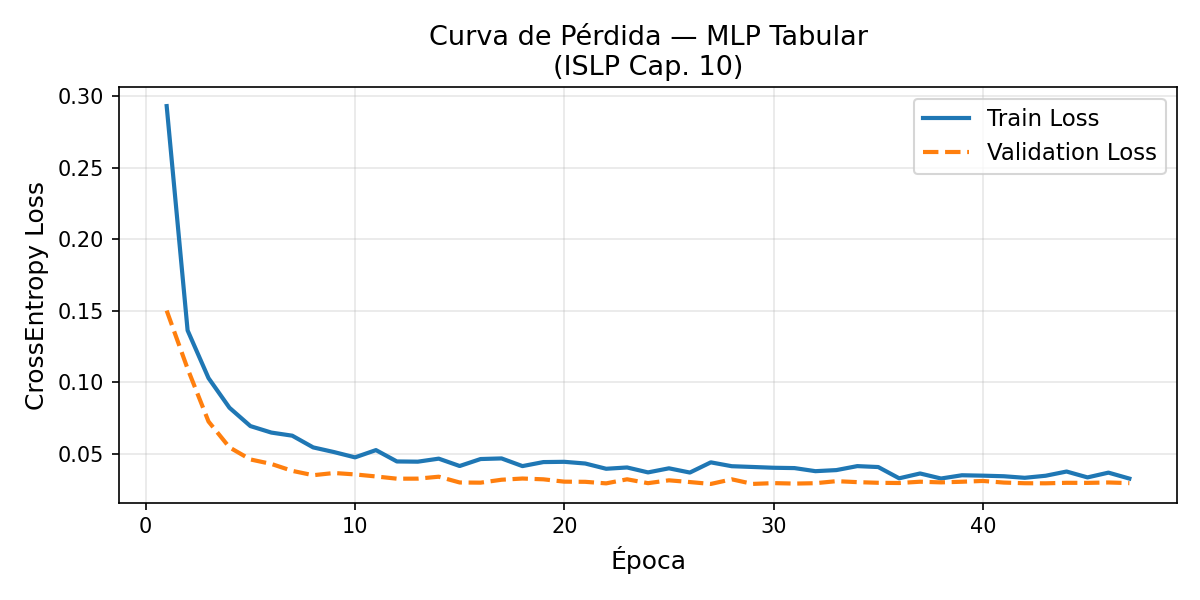
\includegraphics[width=0.82\textwidth]{loss_tabular.png}
  \caption{Curva de pérdida (entropía cruzada) del MLP sobre el conjunto
    de datos tabulares. Línea continua: pérdida de entrenamiento; línea
    discontinua: pérdida de validación.}
  \label{fig:loss_tabular}
\end{figure}

\subsection{Métricas de evaluación}

La Tabla~\ref{tab:metricas_mlp} reporta las métricas sobre el conjunto
de prueba. Test con 968 patrones reales.

\begin{table}[H]
  \centering
  \caption{Métricas de clasificación del MLP sobre el conjunto de
    prueba (968 instancias). Se reporta el promedio binario y ponderado
    dado el desbalance de clases (ratio 17.6:1).}
  \label{tab:metricas_mlp}
  \setlength{\tabcolsep}{10pt}
  \renewcommand{\arraystretch}{1.25}
  \begin{tabular}{lcccc}
    \toprule
    \textbf{Clase / Agregado} & \textbf{Accuracy}
      & \textbf{Precision} & \textbf{Recall} & \textbf{F1-Score} \\
    \midrule
    Clase 1 (mayoritaria, $n=916$) & --- & 0.9919 & 0.9934 & 0.9927 \\
    Clase 2 (minoritaria, $n=52$)  & --- & 0.9020 & 0.8846 & 0.8932 \\
    \midrule
    Global (binary avg)   & \textbf{0.9886} & 0.9020 & 0.8846 & 0.8932 \\
    Global (macro avg)    & ---             & 0.9470 & 0.9390 & 0.9430 \\
    Global (weighted avg) & ---             & 0.9880 & 0.9886 & 0.9883 \\
    \bottomrule
  \end{tabular}
\end{table}

El modelo alcanza un \textbf{Accuracy global del 98.86\%}.
Como advierte \citet[Cap.~4]{islp2023}, en presencia de clases
desbalanceadas el Accuracy puede ser engañoso; por ello se reportan
también Precision, Recall y F1-Score.

% =====================================================================
\section{Resultados: Componente de Imágenes (CNN)}
\label{sec:resultados_imagenes}
% =====================================================================

\subsection{Curva de pérdida}

La Figura~\ref{fig:loss_cnn} ilustra la evolución de la pérdida y
la exactitud por época. La pérdida inicial alta ($\Loss_1 = 10.44$,
típica de pesos aleatorios) desciende bruscamente en las primeras
cinco épocas y converge al mínimo de validación $\Loss^* = 0.1276$
en la época 28.

\begin{figure}[H]
  \centering
  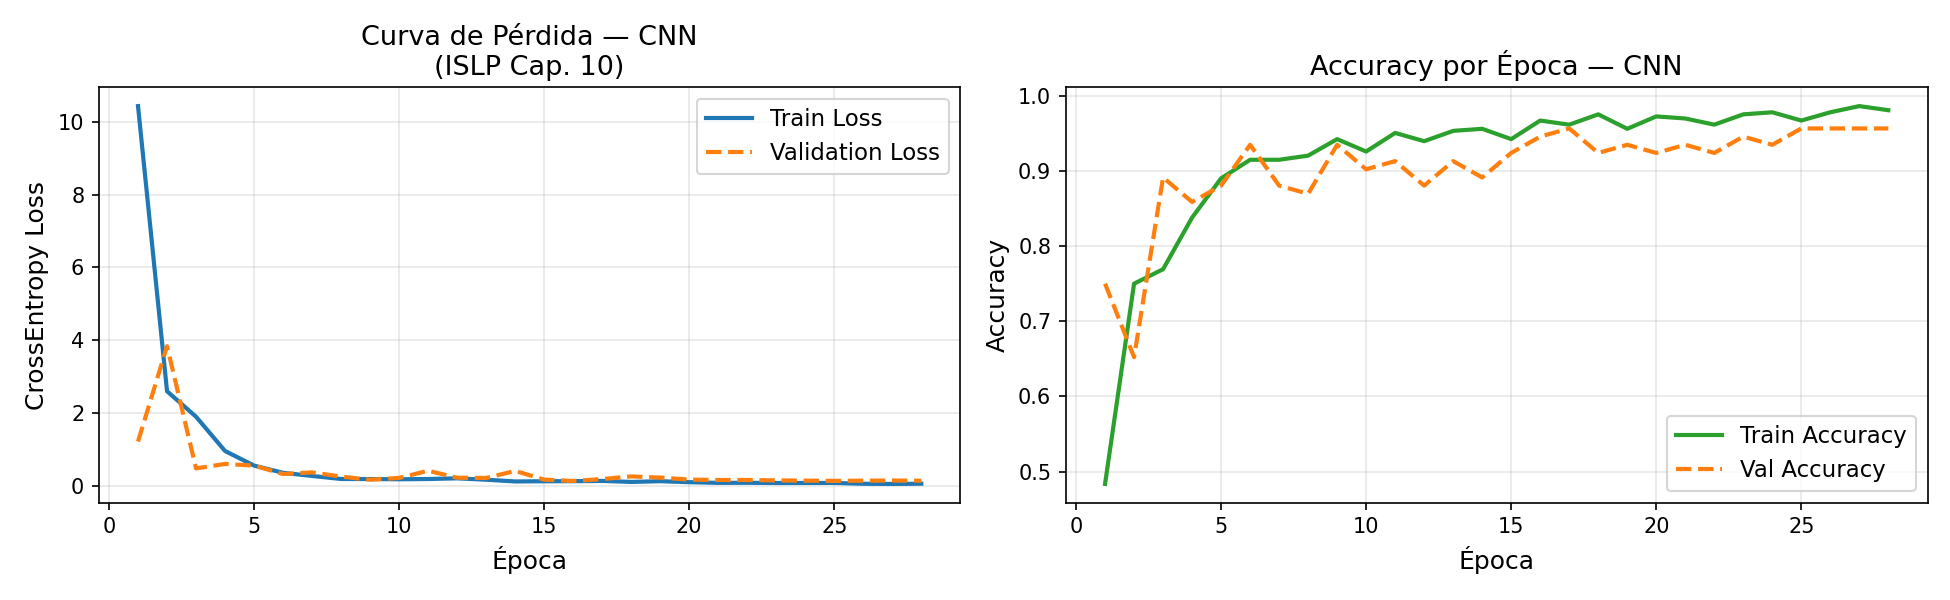
\includegraphics[width=0.95\textwidth]{loss_cnn.png}
  \caption{Evolución de la CNN durante el entrenamiento.
    \textit{Izquierda}: entropía cruzada por época.
    \textit{Derecha}: accuracy en validación por época.}
  \label{fig:loss_cnn}
\end{figure}

\subsection{Accuracy y matriz de confusión}

La CNN alcanzó una \textbf{Accuracy global del 94.57\%} sobre las 92
imágenes de prueba. La Figura~\ref{fig:conf_matrix} muestra la matriz
de confusión en conteos absolutos y normalizada por clase.

\begin{figure}[H]
  \centering
  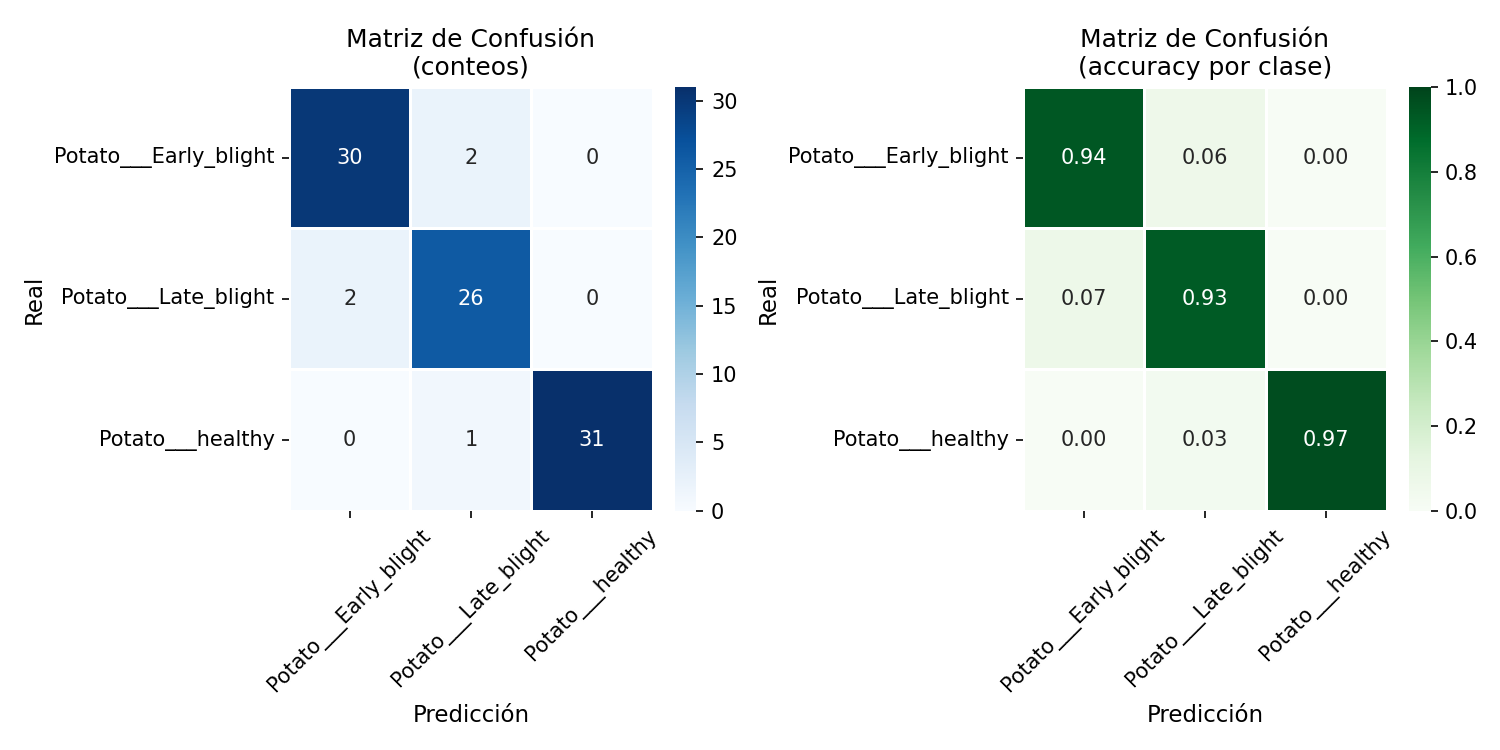
\includegraphics[width=0.90\textwidth]{conf_matrix.png}
  \caption{Matriz de confusión de la CNN sobre el conjunto de prueba.
    \textit{Panel izquierdo}: conteos absolutos.
    \textit{Panel derecho}: accuracy por clase normalizada por fila.}
  \label{fig:conf_matrix}
\end{figure}

\begin{table}[H]
  \centering
  \caption{Métricas de clasificación de la CNN por clase (92 imágenes).}
  \label{tab:metricas_cnn}
  \setlength{\tabcolsep}{9pt}
  \renewcommand{\arraystretch}{1.25}
  \begin{tabular}{lcccc}
    \toprule
    \textbf{Clase} & \textbf{Acc.\ por clase}
      & \textbf{Precision} & \textbf{Recall} & \textbf{F1-Score} \\
    \midrule
    \textit{Early Blight} & 0.9375 & 0.9375 & 0.9375 & 0.9375 \\
    \textit{Late Blight}  & 0.9286 & 0.9000 & 0.9286 & 0.9141 \\
    \textit{Healthy}      & 0.9688 & 1.0000 & 0.9688 & 0.9841 \\
    \midrule
    \textbf{Macro avg}    & ---    & 0.9458 & 0.9449 & 0.9452 \\
    \textbf{Weighted avg} & \textbf{0.9457} & 0.9457 & 0.9457 & 0.9453 \\
    \bottomrule
  \end{tabular}
\end{table}

La clase \textit{Healthy} obtuvo Precision perfecta (1.000): el modelo
nunca clasificó una hoja sana como enferma. Las confusiones más
frecuentes ocurren entre \textit{Early Blight} y \textit{Late Blight},
enfermedades con síntomas foliares visualmente similares.

% =====================================================================
\section{Análisis y Conclusiones}
\label{sec:conclusiones}
% =====================================================================

\subsection{Análisis del rendimiento}

\textbf{Importancia de la normalización (Cap.~2 y 10).}
El MLP tabular se beneficia directamente de \texttt{StandardScaler}.
Con 5 variables en escalas potencialmente distintas, la ausencia de
normalización habría generado gradientes desbalanceados.
\citet[Sec.~10.9.1]{islp2023} enfatizan que normalizar las entradas
es un paso obligatorio: las redes neuronales son sensibles a la escala
de las entradas (al igual que Ridge y Lasso son afectadas).

\textbf{Aumento de datos como regularización (Cap.~10).}
La CNN obtuvo 94.57\% con solo 364 imágenes, resultado notable para un
dataset reducido. Esto se atribuye al aumento de datos, que
\citet[Sec.~10.3.4]{islp2023} describen como una forma de
regularización que enriquece el conjunto de entrenamiento con
perturbaciones realistas.

\textbf{Compromiso sesgo-varianza y early stopping (Cap.~2 y 10).}
La cercanía entre las curvas de pérdida indica que el \textit{early
stopping} ubicó los modelos en el punto óptimo del
\textit{bias-variance tradeoff} (Ecuación~\eqref{eq:bias_variance}).
Según \citet[Sec.~10.8]{islp2023}, detener el gradiente estocástico
antes de la interpolación completa actúa como regularización efectiva.

\textbf{Desbalance de clases y métricas (Cap.~4).}
El menor rendimiento del MLP sobre la clase minoritaria (F1 = 0.893
frente a 0.993) ilustra el problema de desbalance de clases.
\citet[Cap.~4]{islp2023} advierten que en estos escenarios el Accuracy
global puede ser engañoso, y recomiendan Precision, Recall y F1-Score.

\subsection{Limitaciones y trabajo futuro}

\begin{itemize}
  \item El dataset de imágenes (456 imágenes) es pequeño para una CNN
    entrenada desde cero. El \textit{transfer learning} con modelos
    preentrenados como ResNet-50 podría mejorar significativamente el
    rendimiento \citep[Sec.~10.9.4]{islp2023}.
  \item La selección de hiperparámetros fue manual. Una búsqueda
    sistemática mediante validación cruzada $k$-fold
    \citep[Cap.~5]{islp2023} permitiría optimizarlos más
    rigurosamente.
  \item El desbalance 17.6:1 en los datos tabulares podría mitigarse
    con SMOTE o ponderación de clases (\texttt{weight} en
    \texttt{CrossEntropyLoss}).
  \item Los árboles de decisión y Random Forest (Cap.~8) constituyen
    una alternativa interpretable al MLP para el componente tabular,
    especialmente útil para identificar las variables predictoras
    más importantes.
\end{itemize}

\subsection{Conclusiones}

Este proyecto demuestra que las redes neuronales profundas,
implementadas con PyTorch bajo los principios estadísticos de
\citet{islp2023}, constituyen herramientas poderosas para problemas
de clasificación en datos tabulares e imágenes. Los factores
determinantes en el éxito fueron: (1)~el preprocesamiento riguroso
(normalización, aumento de datos), (2)~la regularización combinada
(Dropout, L2, early stopping), y (3)~la elección de activaciones ReLU,
que mitigan el gradiente evanescente. Los resultados obtenidos validan
la metodología y los temas estudiados durante el curso.

% =====================================================================
%  BIBLIOGRAFÍA
% =====================================================================
\newpage
\bibliography{referencias}

\end{document}
